
\subsection{Ejercicios}
\begin{itemize}
 \item 
\textbf{Ejercicio 4}  Completar la implementación del scheduler Round-Robin implementando los
metodos de la clase SchedRR en los archivos sched rr.cpp y sched rr.h. La implementaci\'{o}n
recibe como primer par\'{a}metro la cantidad de n\'{u}cleos y a continuaci\'{o}n los valores de sus
respectivos quantums. Debe utilizar una \'{u}nica cola global, permitiendo ası la migraci\'{o}n de
procesos entre n\'{u}cleos.
\item \textbf{Ejercicio 5} Disene un lote con 3 tareas de tipo TaskCPU de 50 ciclos y 2 de tipo TaskConsola
con 5 llamadas bloqueantes de 3 ciclos de duraci\'{o}n cada una. Ejecutar y graficar la simulaci\'{o}n
utilizando el scheduler Round-Robin con quantum 2, 10 y 50.\\
Con un cambio de contexto de 2 ciclos y un solo n\'{u}cleo calcular la latencia, el waiting
time y el tiempo total de ejecuci\'{o}n de las cinco tareas para cada quantum. 
¿En cual es mejor cada uno? ¿Por qu\'{e} ocurre esto?
\item \textbf{Ejercicio 6} Grafique el mismo lote de tareas del ejercicio anterior para el scheduler FCFS.
Haciendo referencia a lo que se observa en los gr\'{a}ficos de este ejercicio y el anterior, explique
las diferencias entre un scheduler Round-Robin y un FCFS.
\item \textbf{Ejercicio 7} El scheduler SchedMistery fue creado por docentes investigadores de nuestra
materia y ha sido destacado en la ultima publicaci\'{o}n de ACM - SIGOPS, Operating Systems
Review. Desde entonces, numerosos investigadores de todo el mundo nos han contactado para
pedirnos su c\'{o}digo fuente. Sin embargo, su c\'{o}digo no aparece en ninguno de los repositorios
de la materia y nadie parece recordar quienes habıan estado detras de su implementaci\'{o}n.
Se les pide experimentar con dicho scheduler (aprovechando que hemos conseguido el c\'{o}di
go objeto) y replicar su funcionamiento en SchedNoMistery. Graficar como maximo tres lotes
de tareas utilizados en los experiementos y explicar en cada uno por separado que caracter\'{i}sticas
de SchedMistery identificaron con ese lote. Nota: El scheduler funciona para un solo
core y toma uno o mas argumentos num\'{e}ricos.
\item \textbf{Ejercicio 8} Implemente un scheduler Round-Robin que no permita la migraci\'{o}n de procesos
entre n\'{u}cleos (SchedRR2). La asignación de CPU se debe realizar en el momento en que se produce la carga 
de un proceso (load). El n\'{u}cleo correspondiente a un nuevo proceso ser\'{} aquel
con menor cantidad de procesos activos totales (RUNNING + BLOCKED + READY).Explique un escenario real 
donde la migraci\'{o}n de n\'{u}cleos sea beneficiosa y uno donde no (mencione
espec\'{i}ficamente que m\'{e}tricas de comparaci\'{o}n vistas en la materia mejorarıan en cada caso).
Disene un lote de tareas en nuestro simulador que represente a cada uno de esos escenarios
y grafique su resultado para cada implementaci\'{o}n. Calcule y compare en cada gr\'{a}fico las
m\'{e}tricas que menciono.

\end{itemize}


\subsection{Resultados y Conclusiones}

\subsubsection[Resolución Ejercicio 4]{Ejercicio 4}
Para desarrollar la implementación del scheduler $Round-Robin$ y que \'{e}ste funcione de una forma correcta
utilizamos una serie de estructuras puntuales. \\
Las mismas son las siguientes:\\
\begin{enumerate}
 \item Una cola global, la cual nombramos $q$, esta contiene los $PID$ de los procesos activos que no est\'{a}n
 bloqueados y en el tope de la misma se encuentra el próximo proceso a correr. Esta cola,
 fue desarrollada para que cuando se desaloje un proceso por finalizar su $quantum$ la misma pase al final de
 la cola y generando el ciclo acorde al comportamiento de este scheduler.
 \item Un vector denominado $cores$, este tiene en su elemento $i$ el pid correspondiente 
 al proceso que está corriendo en el core $i+1$. Inicializamos todos los elementos en -1, esto
corresponde a la Idle Task, de esta forma reconocemos que no se cargaron procesos en los núcleos.
\item Un vector $quantum$: el mismo guarda en la posici\'on $i$ el quantum que se dispuso a cada núcleo.
\item Un vector $quantumActual$ aqu\'{\i} guardaremos la cantidad de ticks que le quedan al proceso
desde que fue cargado en el core.
\item Una lista de $bloqueados$: esta tendr\'{a} los procesos que se bloquearon cuando estaban corriendo.
\end{enumerate}

Estas estructuras nos permiten determinar para cada tarea, cuándo, y cuánto 
de su quantum consumieron de forma que podamos desalojarla correctamente.\\

A su vez, tomamos ciertas decisiones en esta implementación:
\begin{itemize}
 \item Si una tarea se encuentra bloqueada cuando se produce el tick del reloj, misma es desalojada
de la cola global, y agregada en una lista de bloqueados. Además, ser\'{a} reseteado el quantum, se le
dará inicio a la próxima tarea que se encuentre ready y cuando el sistema operativo nos envie una
señal de unblock, la tarea desalojada regresará al final de la cola global.

\end{itemize}

\begin{center}

    
	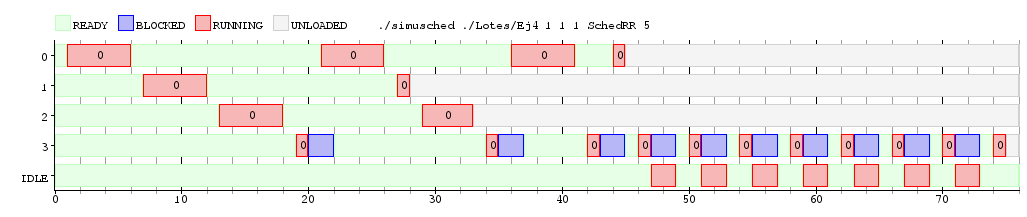
\includegraphics[width=450pt]{./Test/Ej4.png}
	{$Gr$\'a$fico 4.1 - Lote 1$ - Scheduler RR - 1 core - 5 quantum}	
 
\end{center}

Se puede ver en el gr\'{a}fico que cada 5 Ticks de reloj se cambia de tareas de manera c\'{\i}clica para mantener 
el fairness lo mas posible con todas las tareas. Salvo cuando una tarea se bloquea que esta es desalojada inmediatamente 
para no desperdiciar tiempo de computo esperando a que esta de desocupe.

\subsubsection[Resolución Ejercicio 5]{Ejercicio 5}

\indent El algoritmo de scheduler \textbf{Round-Robin} tiene como caracter\'istica asignar a todas las tareas 
un determinado tiempo m\'aximo de procesamiento, a esto se lo llama $quantum$. \\
\indent Este tiempo esta definido para cada n\'ucleo en particular, dependiendo de en cu\'al de ellos est\'en 
ejecutando los procesos, se les asignar\'a el respectivo tiempo m\'aximo.\\
\indent Otra caracter\'istica del \textbf{Round-Robin} es que las tareas se encolan y se ejecutan c\'iclicamente. 
Osea que cuando se deja de ejecutar, si no termin\'o su ejecuci\'on, la tarea se encolar\'a al final de la lista. 
Como elecci\'on de diseño, elegimos que se use una cola global para todos los procesadores, aunque tambi\'en
se podr\'ia tener una cola para cada n\'ucleo. \\
\indent A su vez, tambi\'en puede ocurrir una tarea no consuma todo su $quantum$. 
Ya sea porque la tarea se bloquea (haciendo uso de dispositivos de entrada/salida) o porque termine su ejecuci\'on.\\
\indent En caso de haber terminado, nuestro algoritmo pone a correr directamente la pr\'oxima tarea de acuerdo al orden 
circular que se estableci\'o y la tarea que finaliz\'o se desalojar\'a por completo y no sera considerada nuevamente. \\
\indent En caso de haberse bloqueado, esta misma dejar\'a de ser considerada hasta que se desbloquee, 
perdiendo el quantum que le quedaba si hubiere. 
Autom\'aticamente, seguir\'a corriendo la pr\'oxima tarea que se encuentre en la cola global. 
Cuando el proceso se desbloquee, ser\'a encolada nuevamente al final de dicha cola.   \\

\indent Para corroborar que el comportamiento era el deseado, nos solicitaron 1 lotes de tareas compuestos por tareas
del tipo $taskConsola$ y $taskCpu$, trabajando con 1 cores y utilizando distintos $quantum$ para cada uno de los mismos.\\

El lote de tareas fue el siguiente:
\begin{verbatim}
                                   *3 TaskCPU 50
                                   *2 TaskConsola 5 3 3
\end{verbatim}

Obteniendo los siguientes resultados:

\begin{center}

    
	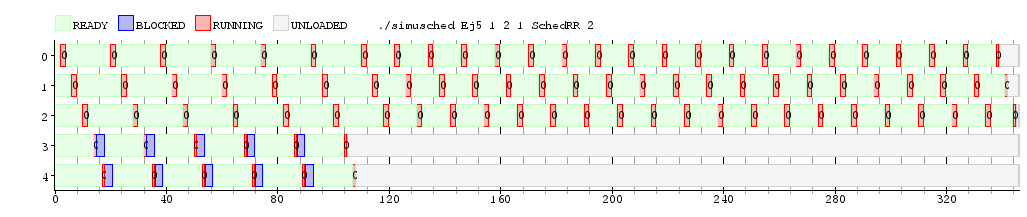
\includegraphics[width=450pt]{./Test/ej5_2.png}
	{$Gr$\'a$fico 5.1 Lote 1$ - Scheduler RR - 1 core - 2 quantum}	
 
\end{center}

\indent Latencia:\
\begin{itemize}
 \item Tarea 0: 2
 \item Tarea 1: 6
 \item Tarea 2: 10
 \item Tarea 3: 14
 \item Tarea 4: 18
 \item PROMEDIO: 10
\end{itemize}
\indent Waiting time:\
\begin{itemize}
 \item Tarea 0: 289
 \item Tarea 1: 292
 \item Tarea 2: 295
 \item Tarea 3: 84
 \item Tarea 4: 87
 \item PROMEDIO: 209,4
\end{itemize}
\indent Tiempo total de ejecuci\'{o}n:\
\begin{itemize}
 \item Tarea 0: 339
 \item Tarea 1: 342
 \item Tarea 2: 345
 \item Tarea 3: 105
 \item Tarea 4: 108
 \item PROMEDIO: 247,8
\end{itemize}

\begin{center}
  	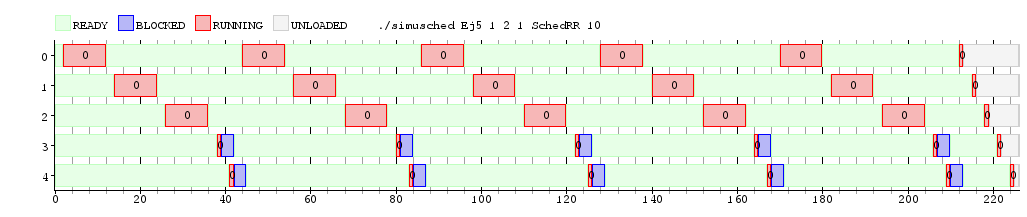
\includegraphics[width=450pt]{./Test/ej5_10.png}
	  {$Gr$\'a$fico 5.2 - Lote 1$ - Scheduler RR - 1 core - 10 quantum}	
\end{center}

\indent Latencia:\
\begin{itemize}
 \item Tarea 0: 2
 \item Tarea 1: 14
 \item Tarea 2: 26
 \item Tarea 3: 38
 \item Tarea 4: 41
 \item PROMEDIO: 24,2
\end{itemize}
\indent Waiting time:\
\begin{itemize}
 \item Tarea 0: 162
 \item Tarea 1: 165
 \item Tarea 2: 198
 \item Tarea 3: 201
 \item Tarea 4: 204
 \item PROMEDIO: 186
\end{itemize}
\indent Tiempo total de ejecuci\'{o}n:\
\begin{itemize}
 \item Tarea 0: 213
 \item Tarea 1: 216
 \item Tarea 2: 219
 \item Tarea 3: 222
 \item Tarea 4: 225
 \item PROMEDIO: 219
\end{itemize}

\begin{center}
  	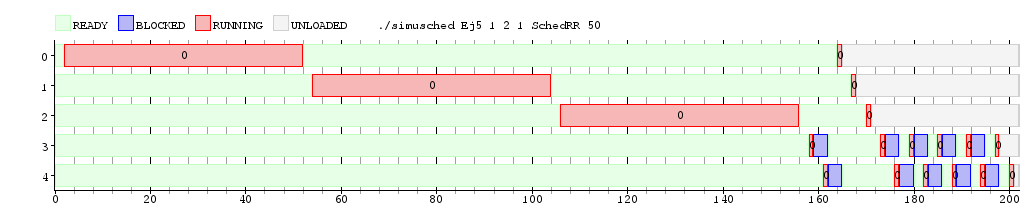
\includegraphics[width=450pt]{./Test/ej5_50.png}
	  {$Gr$\'a$fico 5.3 - Lote 1$ - Scheduler RR - 1 core - 50 quantum}	
\end{center}

\indent Latencia:\
\begin{itemize}
 \item Tarea 0: 2
 \item Tarea 1: 54
 \item Tarea 2: 106
 \item Tarea 3: 158
 \item Tarea 4: 161
 \item PROMEDIO: 96,2
\end{itemize}
\indent Waiting time:\
\begin{itemize}
 \item Tarea 0: 114
 \item Tarea 1: 117
 \item Tarea 2: 120
 \item Tarea 3: 177
 \item Tarea 4: 180
 \item PROMEDIO: 141,6
\end{itemize}
\indent Tiempo total de ejecuci\'{o}n:\
\begin{itemize}
 \item Tarea 0: 165
 \item Tarea 1: 168
 \item Tarea 2: 171
 \item Tarea 3: 198
 \item Tarea 4: 201
 \item PROMEDIO: 180,6
\end{itemize}

\indent
\begin{itemize}
 \item El caso con mejor latencia es el primer experimento, esto se debe al escaso quantum que se le otorga a cada tarea
 permitiendoles ejecutar por primera vez r\'{a}pidamente.
 \item El 3er experimento tiene el mejor waiting time, esto se debe a su alto quantum. Debido a que el quantum es muy elevado 
 se desperdicia la menor cantidad de ticks de reloj en cambio de contexto.
 \item Igual que en el caso anterior como el 3er experimento es el que menos ticks pierde por cambio de contexto debido al 
 alto quantum, esta es la que menos tiempo de ejecuci\'{o}n tiene.
\end{itemize}


\indent Se puede observar el cambio de tareas cíclico tanto porque terminaron su quantum o porque se bloquearon.\\


\indent Luego de estos experimentos pudimos observar ciertos puntos del comportamiento del Round-Robin:\\
\begin{itemize}
\item  Carácter circular del algoritmo.
\item  Desalojo de las tareas cuando se bloquean o terminan y la inmediata asignación del núcleo a la siguiente tarea en caso de existir alguna.
\item  Libre de inanición.
\item  Una tarea bloqueada es ignorada por el scheduler hasta que se desbloquee.
\end{itemize}

\indent Finalmente, dado su carácter circular y equitativo, podemos afirmar que todas las tareas que 
estén en condiciones de correr serán ejecutadas y ninguna será negada de tiempo de procesamiento.\\


\subsubsection[Resolución Ejercicio 6]{Ejercicio 6}

El lote de tareas solicitado fue el siguiente:
\begin{verbatim}
                                   *3 TaskCPU 50
                                   *2 TaskConsola 5 3 3
\end{verbatim}

Obteniendo los siguientes resultados:

\begin{center}
  	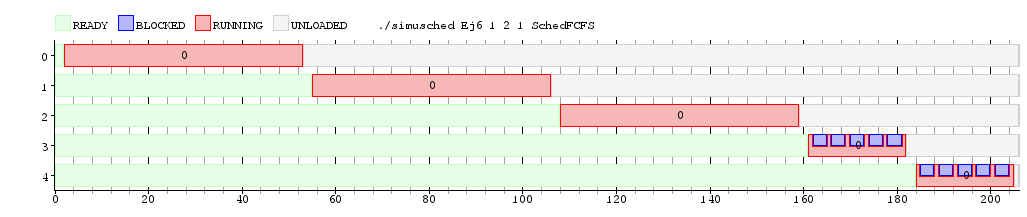
\includegraphics[width=450pt]{./Test/ej6.png}
	  {$Gr$\'a$fico 6.1 - Lote 1$ - Scheduler FCFS - 1 core}	
\end{center}

\indent A modo de an\'alisis, hemos obtenido las siguientes conclusiones:\\


\begin{itemize}
 \item Un scheduler FCFS corre una tarea hasta que esta termina a diferencia de uno Round-Robin 
que las va intercambiando otorg\'{a}ndole un tiempo equitativo a cada tarea.
\item Para que Round-Robin sea considerablemente mas eficiente que FCFS el quantum debe ser 
lo suficientemente alto para no tenes altos valores de waiting-time durante los cambios de 
contexto pero no demasiado alto sino se comporta igual que un scheduler FCFS.
\item Si se da el caso anterior el scheduler Round-Robin es eficiente en t\'{e}rminos 
de latencia en comparaci\'{o}n con FCFS.
\end{itemize}


\subsubsection[Resolución Ejercicio 7]{Ejercicio 7}

\indent En este punto se nos solicit\'{o} experimentar con el c\'{o}digo objeto de un 
SchedMistery y a partir de los mismos, realizar una r\'{e}plica del mismo.\\

A continuacio\'{o}n, expondremos tres experimentos de los cuales sacamos ciertas particularidades que presenta este Scheduler.\\

Con un lote de tareas compuesto por:\\

\begin{verbatim}
 @5:
TaskCPU 20
@0:
TaskCPU 7
TaskConsola 5 2 2
@:8
TaskConsola 4 2 3
\end{verbatim}

Obteniendo lo siguiente:
\begin{center}
    	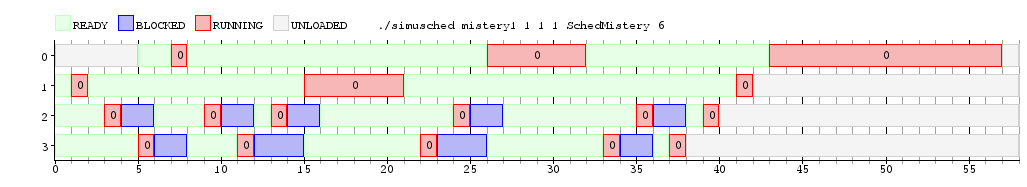
\includegraphics[width=450pt]{./Test/ej7_1.png}
	{$Gr$\'a$fico 7.1 - Lote 1$ - Sched Mistery - 1 core - Quantum = 6}	
 \end{center}
 
De aqu\'{\i}, pudimos abstraer que, una tarea al bloquearse es desalojada y cuando la misma se desbloquea, el scheduler, le da
una prioridad otorg\'{a}ndole quantum = 1 para que vuelva a correr y luego volver a encolarla en un orden cclico similar al de Round-Robin.\\

Con el siguiente lote:\\

\begin{verbatim}
              TaskCPU 20
              TaskCPU 10
              @20:
              TaskCPU 15
\end{verbatim}

Obteniendo lo siguiente:\\
\begin{center}
    	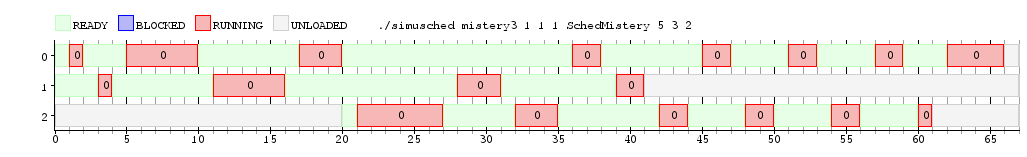
\includegraphics[width=450pt]{./Test/ej7_3.png}
	{$Gr$\'a$afico 7.2 - Lote 2$ - Sched Mistery - 1 core - Quantum = 5 3 2}	
 \end{center}
 
De aqu\'{\i}, pudimos observar, la existencia de una prioridad a tareas $mas$ $nuevas$, ya que al llegar la misma y estar ready, es
la proxima a correr por el scheduler, y con un quantum igual a la sumatoria de los quantum ya pasados hasta el momento de ser cargada.\\
Se puede apreciar tambie\'{e}n un orden ciclico del mismo, y luego de dar esta prioridad mencionada por \'{u}nica vez, dicha tarea es encolada con un orden c\'{\i}clico
respetando el mismo quantum que el resto de las tareas.\\
Adem\'{a}s, se puede observar distintos valores de quantums, inicialmente todos con 1, y luego, por cada vuelta c\'{\i}clica los mismos van cambiando dependiendo del valor recibido
como par\'{a}metro.(En nuestro experimento, por ej, los valores fueron 5 3 y 2)\\

\indent En conclusi\'on:\\


\begin{itemize}
 \item Se puede observar un caracter c\'{\i}clico con posibilidad de varios quantums distintos, los cuales van cambiando
 acorde a las vueltas c\'{\i}clicas que da el scheduler.
 \item Prioridad para tareas bloqueantes (al ser desbloqueada es la primera en cargar otorg\'{a}ndole quantum = 1)
 \item Prioridad para tareas m\'as recientes (al llegar la misma y estar ready esta pasa a ser la pr\'{o}xima en correr con un quantum igual
 a la sumatoria de los quantums ya transcurridos hasta el momento)
\end{itemize}


Para desarrollar la implementación del scheduler $No$ $Mistery$ y que este funcione de una forma correcta
utilizamos una serie de estructuras puntuales. \\
Las mismas son las siguientes:\\
\begin{enumerate}
 \item Una cola, la cual nombramos $q$, esta contiene los $PID$ de los procesos activos que no estan
 bloqueados y en el tope de la misma se encuentra el próximo proceso a correr. Esta cola,
 fue desarrollada para que cuando se desaloje un proceso por finalizar su $quantum$ la misma pase al final de
 la cola y generando el ciclo acorde al comportamiento de este scheduler.
 \item Un vector denominado $quantum$, este tiene en su elemento $i$ el quantum correspondiente a
a la ronda c\'iclica que se esta corriendo en el momento. Inicializamos todos los elementos con los valores que recibimos
como par\'ametro.
\item Un cola nombrada como $desbloqueados$ y como el nombre lo indica, tendr\'a las tareas que se desbloquearon y estan
listas para correr.
\item Un map de pair\textless \ int, int\textgreater \ $pid_quantum$ aqui guardaremos en el primer elemento el pid y en el segundo el quantum con el que 
iniciar\'a a correr, ya sea 1 o la sumatoria de quantums ya corridos hasta el momento que la tarea es cargada.
desde que fue cargado en el core.
\item Un map de pair\textless \ int, int\textgreater \ $pid_Tarde$ este nos indicar\'a dependiendo el pid si la tarea fue cargada al iniciar el lote o si llego mas 
tarde
\item Un map de pair\textless \ int, int\textgreater \ $pid_Bloqueado$ este map nos dir\'a si la tarea estuvo bloqueada o no.
\item Un entero $pidInicial$ en esta variable guardaremos el pid de la primer tarea de nuestro orden ciclico, esto
nos servira para que en cada rueda al finalizar y le vuelva a tocar a el pid inicial aumentemos el contador $contQuantumPasados$
y actualizemos el indice del vector $quantum$
\item Un entero $contQuantumPasados$ que como mencionamos anteriormente nos da la cantidad de vueltas completas que se dieron
\item Un entero $quantumActual$ en el cual almacenaremos el valor de quantum que tiene en el momento la tarea que esta corriendo
\end{enumerate}

 De esta manera, con estas estructuras nos permiten determinar para cada tarea, cuándo, y cuánto 
de su quantum consumieron de forma que podamos desalojarla correctamente.\\

Obteniendo las prioridades caracter\'isticas de dicho scheduler tanto para la tarea bloqueadas como para las que llegan "tarde".\\
Con nuestro map de $pid_Tarde$ y $pid_Bloqueado$ podremos reordenar nuestra cola $q$ con la cual realizamos la ejecuci\'on ciclica de nuestro
sched logrando el orden deseado y particular.\\

\subsubsection[Resolución Ejercicio 8]{Ejercicio 8}

La idea principal de esta nueva versi\'{o}n de $Round-Robin$ se centraliza en que no permita migraci\'{o}n entre
cores, esto se basa principalmente en utilizar una cola para cada núcleo por separado, y en cada
cola respectiva se encolar\'{a}n las tareas que fueron asignadas inicialmente a cada n\'ucleo.\\
Para desarrollar este tipo de algoritmo, el cual denominaremos $RR2$, utilizamos estructuras
puntuales, enunciadas a continuación:\\
\begin{itemize}
 \item Un vector $quantum$ y otro $quantumActual$, los cuales siguen cumpliendo la misma funci\'{o}n que
 en Round-Robin 1.
 \item Un vector de colas denominado $colas$, en el cual, en la posición $i$ encontraremos la cola correspondiente
 a ese núcleo de procesamiento.
 \item Un diccionario de $Bloqueados$, donde la clave contendr\'{a} el número de core, y en definición
 la tareas bloqueadas de ese core. Esto nos beneficiar\'{a} cuando haya que reubicarla en la cola de procesos ready.
 \item Un vector de enteros $cantidad$, que como la palabra lo define, tendrá en cada posición $i$ 
 la totalidad de las tareas, ya sea bloqueadas, activas o en estado ready que tiene asignado ese core, benefici\'{a}ndonos
 la determinación del núcleo al que se le asignará la tarea al momento de cargarla.
\end{itemize}
Cuando se carga una tarea, previamente, se chequeará que core tiene menor cantidad de procesos totales asignados (
aqu\'{\i} es donde el vector $cantidad$ entra en juego). Una vez que se obtiene este n\'{u}cleo, se agrega 
la tarea a la cola correspondiente y se actualiza la cantidad sumando una unidad.\\
\indent Al bloquearse un proceso, se define una nueva entrada en el diccionario $bloqueados$ con el
pid y el n\'{u}cleo correspondiente. De esta forma, al desbloquearse, colocamos la tarea en la cola del core
correspondiente y eliminamos la entrada del diccionario. Así logramos resolver el inconveniente de la nula
migración entre n\'{u}cleos.\\
\indent Finalmente, cuando una tarea finaliza, la quitamos y descontamos una unidad a la posición $i$ del vector
$cantidad$. Esta es la única vez, en la cual se descuenta. Aunque una tarea se bloquee, la misma
seguirá contando en el vector. De esta forma se cumplirá, que las tareas son asignadas a los cores
con menor cantidad de tareas.\\
Luego de realizar dicha implementación, en comparación al Round-Robin original, hemos conjeturado 
las siguientes hipótesis:

\begin{enumerate}
\item Comportamiento menos eficiente en el RR2 con respecto al paralelismo, ya que al no permitir
migración de n\'ucleos este se pierde.
\item Comportamiento más eficiente en el RR2 con lotes de tareas que se bloquean un gran n\'{u}mero
de veces. Esto surge ya que el Round-Robin original, es m\'as proclive a realizar cambios de contexto con la posibilidad
de darse un cambio de core.
\end{enumerate}
 
 Procedemos a demostrar la primer conjetura:\\
 
 \textbf{Comportamiento menos eficiente en el RR2 con respecto al paralelismo, ya que al no permitir
migración de núcleos este lo pierde}\\

Un ejemplo de esto, en la vida real ser\'ia, estar corriendo testeos de software y al mismo tiempo analizando
algoritmos de alta complejidad para demostraciones matem\'{a}ticas.\\

Un ejemplo de los lotes utilizados que demuestra esto fue el siguiente:\\

\begin{verbatim}
                                     TaskCPU 40
                                     TaskCPU 15
                                     TaskCPU 50
                                     TaskCPU 30
                                     TaskCPU 50
\end{verbatim}

Obteniendo los siguientes datos relevantes:\\

\begin{center}
    	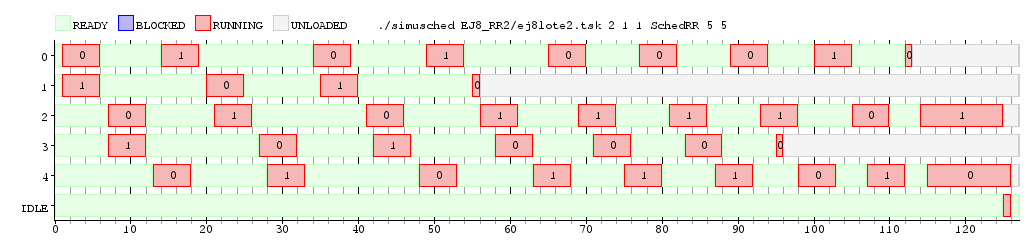
\includegraphics[width=450pt]{./EJ8_RR2/dif10corerr.png}
	{$Gr$\'a$fico 8.1 -Lote 3$ - Round Robin - 2 core - Quantum = 5 - cambio de contexto = 1}	
 \end{center}
 
 \begin{center}
    	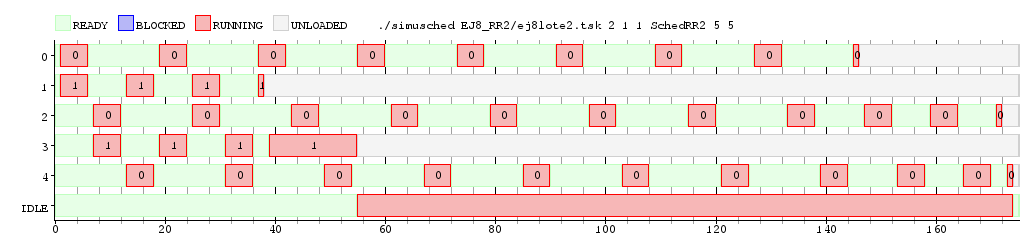
\includegraphics[width=450pt]{./EJ8_RR2/dif10corerr2.png}
	{$Gr$\'a$fico 8.2 - Lote 3$ - Round Robin 2 - 2 core - Quantum = 5 - cambio de contexto = 1}	
 \end{center}
 
 Se puede ver en estos diagramas como la implementación del Round Robin original trabaja
 mejor finalizando la ejecución de las tareas hasta 50 milisegundos antes.\\
 Esto se da por la falta de paralelismo de el RR2 ya que al ser asignados los procesos
 a cada core, cuando uno de los dos finaliza, este queda ocioso ya que no existe la
 posibilidad de migrar  procesos.\\
 
 Luego, el RR2 resulta beneficioso:
 
 \textbf{Comportamiento mas eficiente en el RR2 con lotes de tareas que se bloquean un gran numero
de veces}

\indent Un ejemplo de esto, puede ser al estar corriendo un juego (en el cual siempre se esta interactuando con el teclado) y
adem\'{a}s estar corriendo algun software.\\

Para esto,un lotes de tareas que ejemplifica lo dicho puede ser el siguiente:\\

\begin{verbatim}
                                     TaskCPU 40
                                     TaskBatch 10  5
                                     TaskCPU 50
                                     TaskBatch 15 8
                                     TaskCPU 10

\end{verbatim}


   \begin{center}
    	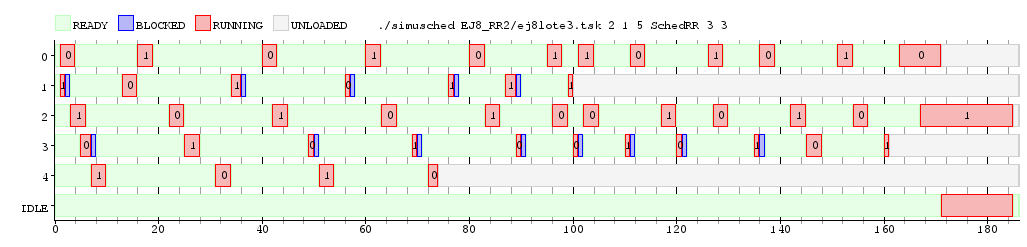
\includegraphics[width=450pt]{./EJ8_RR2/dif5corerr.png}
	{$Gr$\'a$fico 8.3 - Lote 3$ - Round Robin - 2 core - Quantum = 3 - cambio de contexto = 1}	
 \end{center}
 
 \begin{center}
    	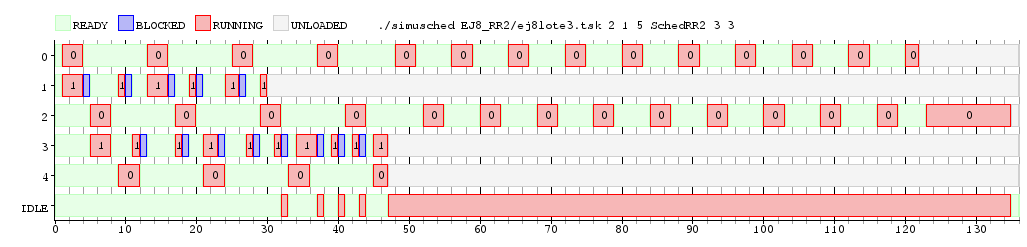
\includegraphics[width=450pt]{./EJ8_RR2/dif5corerr2.png}
	{$Gr$\'a$fico 8.4 - Lote 3$ - Round Robin 2 - 2 core - Quantum = 3 - cambio de contexto = 1}	
 \end{center}

 Se puede observar por los diagramas como el RR2 tiene una mejor performance en este estilo
 de lotes llegando a finalizar las ejecuciones hasta 50 milisegundos antes que el Round-Robin
 original.\\
 Como el Round-Robin original tiene pérdida de tiempo con el cambio de contexto y
 migración de tareas este empeora su performance en comparación al RR2 que no admite
 este tipo de migración es notorio la superioridad en relación a nuestra conjetura.\\
 
 Las m\'{e}tricas que m\'{a}s tuvimos en cuenta a la hora de analizar en que casos tiene mejor performance 
 cada scheduler fueron waiting time y turnaround y throughput. En el primer caso se ve que el scheduler round-robin 2 
 al no migrar las tareas de n\'{u}cleo dado un instante de tiempo un n\'{u}cleo ya queda ocioso haciendo que el 
 otro n\'{u}cleo tenga que encargarse de todas las tareas restantes lo que aumenta considerablemente el 
 waiting time de cada tarea por consiguiente su turnaround y el througput del sistema.
 Lo que sucede en el 2do caso es que el tiempo que tarda un n\'{u}cleo en hacer un cambio de contexto es sumamente 
 negativo para el waiting time general del round-robin
 Podemos concluir luego de estas demostraciones que, el Round-Robin original es \'{a}mpliamente
 superior desde el punto de vista de la performance que se obtiene al trabajar con tareas
 que demanden mucho uso del CPU, mientras que el RR2 es \'{a}mpliamente mejor cuando se utilicen
 tareas que se bloqueen por un tiempo considerable.\\
 
 

